\section{Integration und Programmierung der Steuerungstechnik \textcolor{gray}{ (Vincent Sonvilla)}}


\subsection{Aufgabenstellung}


\subsection{Tia-Portal Grundlagen}

Tia Portal (Totally Integrated Automation Portal) ist die zentrale Software von Siemens zur Programmierung, Konfiguration und Diagnose von Automatisierungssystemen. Es ermöglicht die Steuerung von SPS (Speicherprogrammierbare Steuerungen), HMI (Bedienpanels) und Antrieben in einer einzigen Umgebung.

    \subsubsection{Allgemeines}

        \paragraph{Arbeitsweise einer SPS} \mbox{} \\
        Eine SPS arbeitet zyklisch. In Abb. \ref{Arbeitsweise_einer_SPS} wird gezeigt wie ein solcher Zyklus aussieht. Bei erstmaligem Starten oder Neustarten der SPS werden zuerst alle Ausgänge, Merker, etc. auf Null gesetzt. Danach startet die zyklische Arbeitsweise. Zuerst wird ein Prozessabbild der Eingänge gemacht. Mit diesen Eingangswerten wird dann das Programm ausgeführt. Anschließend wird ein Prozessabbild der Ausgänge gemacht. Dieses wird dann an die Ausgänge übergeben. Danach beginnt der Zyklus von vorne. \cite{Arbeitsweise_der_SPS}
        \begin{figure}[h]
            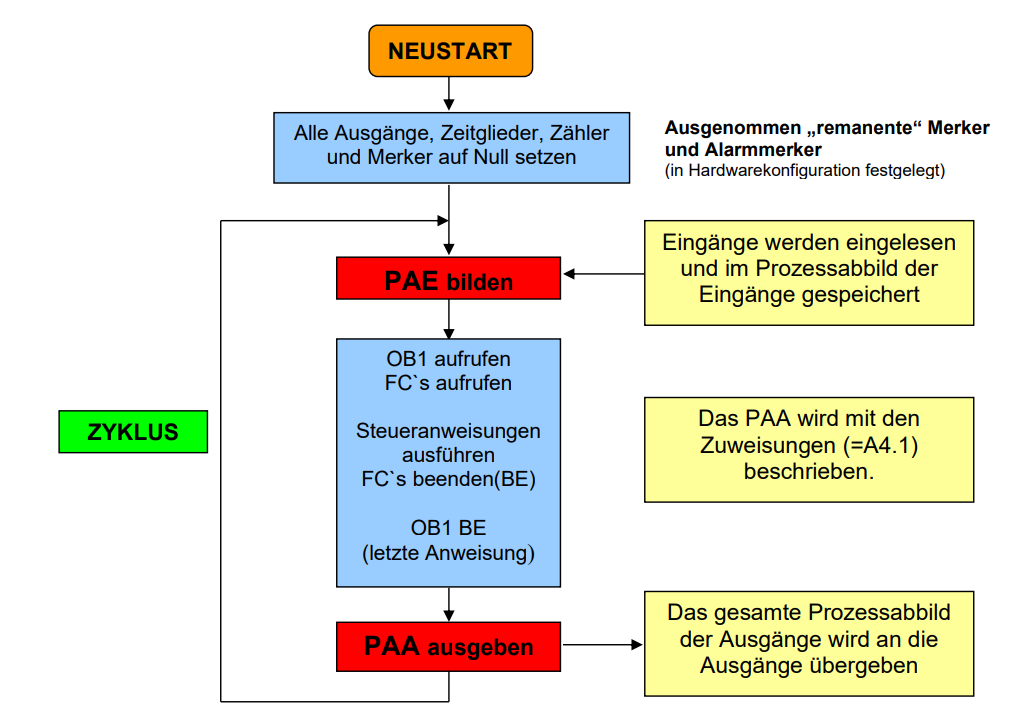
\includegraphics[width=0.9\textwidth]{Sonne/Arbeitsweise_einer_SPS.png}
            \caption{Arbeitsweise einer SPS \cite{Arbeitsweise_der_SPS}}
            \label{Arbeitsweise_einer_SPS}
        \end{figure}

        noch Datentypen, ... maybe

    \subsubsection{Programmbausteine}
    
    In TIA Portal werden Programmbausteine genutzt, um Steuerungsprogramme modular und strukturiert zu gestalten. Dadurch werden Programme übersichtlicher, wiederverwendbar und effizienter. Es gibt unterschiedliche Arten von Programmierbausteinen:

    \begin{itemize}
        \item[1.] \textbf{OB(Organisationsbausteine)} \\
            Organisationsbausteine werden verwendet um das Anwenderprogramm hierarchisch zu strukturieren. Auch für OBs stehen,wie in Abb. \ref{Organisationsbausteine} gezeigt, unterchiedliche Bausteine zur Verfügung:
            \begin{figure}[h]
                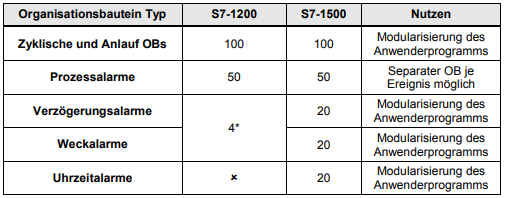
\includegraphics[width=\textwidth]{Sonne/Tia-Portal_Organisationsbausteine.png}
                \caption{Organisationsbausteine \cite{Programmierleitfaden_für_S7-1500}}
                \label{Organisationsbausteine}
            \end{figure}

            Organisationsbausteine steuern unterschidiedliche Vorgänge:
            \begin{itemize}
                \item Anlaufverhalten der Steuerung
                \item Zyklische Programmbearbeitung
                \item Alarmgesteuerte Programmbearbeitung
                \item Behandlung von Fehlern
            \end{itemize}
            Werden in einem Programm mehrere OBs aufgerufen, so werden die OBs in aufsteigender Reihenfolge der OB-Nummer abgearbeitet. 
            \cite{Programmierleitfaden_für_S7-1500}

        \item[2.] \textbf{FC(Funktionen)} \\
            Funktion haben keinen zyklischen Datenspeicher, deswegen können Bausteinparameter nicht bis zum nächsten Aufruf gespeichert werden. Darum müssen Funktionen bei jedem Aufruf mit Aktualparametern versorgt werden. Um kein zufälliges Verhalten enstehen zu lassen sind die Werte immer mit einem Defaultwert vorbelegt. Will man die Daten einer Funktion dauerhaft speichern, so muss man einen globalen Datenbaustein verwenden.\\
            Funktionen werden verwendet, um häufig wiederkehrende Anwendungen durchzuführen.
            \cite{Programmierleitfaden_für_S7-1500}
            
        \item[3.] \textbf{FB(Funktionsbausteine)} \\
            Im Gegensatz zu Funktionen haben Funktionsbausteine einen zyklischen Datenspeicher -Instanz DB-, in welchem Werte dauerhaft gespiechert werden.Dadurch behalten statische Variablen ihren Wert von Zyklus zu Zyklus. Wie bei Funktionen sind die Werte mit einem Defaultwert vorbelegt.\\
            Funktionsbausteine können genutzt werden, um Unterprogramme für unterschiedliche Anwendungen zu erstellen. Außerdem werden sie genutzt um das Anwenderprogramm zu strukturieren. Bei mehrfacher Verwendung von Funktionsbausteinen empfiehlt sich die Verwendung von Multiinstanz-DBs.
            \cite{Programmierleitfaden_für_S7-1500}
        
        \item[4.] \textbf{Global-DB(Datenbausteine)} \\
            Globale Datenbausteine speichern variable Daten, die dem kompletten Programm zur Verfügung stehen. Wie in Abb.\ref{Zugriff auf Global-DB} ersichtlich, bedeutet das ,dass alle Bausteine Zugriff auf den Global-DB haben.

            \begin{figure}[h]
                \centering
                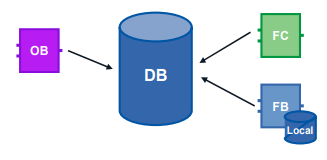
\includegraphics{Sonne/Zugriff_auf_Global-DBs.png}
                \caption{Zugriff auf Global-DB \cite{Programmierleitfaden_für_S7-1500}}
                \label{Zugriff auf Global-DB}
            \end{figure}

            In Globalen Datanbausteinen können jegliche Datentypen genutzt werden.\\
            Globale DBs werden verwendet, wenn Daten in verschiedenen Programmteilen bzw. Bausteinen benötigt werden.
            \cite{Programmierleitfaden_für_S7-1500}

        \item[5.] \textbf{Instanzen} \\
            Wird ein Funktionsbaustein aufgerufen, so nennt man das Instanz. Die Daten der Instanz, werden im sogenannten Instanzdatenbaustein gespeichert. Instanz-DBs werden automatisch nach den Vorgaben des Funktionsbausteins erzeugt und können somit nicht direkt geändert werden. Der Instanz-DB hat einen dauerhaften Speicher, welcher die Schnittstellen Input, Output, InOut sowie Static beihaltet. Zusätzlich besitzt der Instanz-DB einen flüchtigen Datenspeicher in dem tempöräre Variablen gespeichert werden. Diese sind dadurch immer nur für einen Zyklus gültig.
            
        \item[6.] \textbf{Multiinstanzen} \\
            Bei Multiinstanzen speichert der Funktionsbausetein seine Daten in den Instanz-DB des übergeordneten Funktionsbaustein. Das heißt es wird in einem FB ein anderer FB aufgerufen. Dieser speichert seine Daten dann im Instanz-Db des Funktionsbausteins, welcher ihn aufgerufen hat. Multiinstanzen helfen das Programm übersichtlicher sowie strukturierter zu halten, da man mehrere Instanzen in einer Instanz vereint.

    \end{itemize}

    \subsubsection{Technologieobjekte}
    Technologieobjekte dienen dazu die Ansteuerung und Handhabung von technischen Funktionen, insbesondere von Motoren, Achsen, etc. zu vereinfachen. Es existieren eine Vielzahl an unterschiedlichen Technologieobjekten. In nachfolgenden Absätzen werden die für das Projekt relevanten Technologieobjekte genauer erklärt.

    \begin{itemize}

        \item[1.] \textbf{Positionierachse (PositioningAxis)} \\
            Dieses Technologieobjekt dienz zur genauen Positionierung einer Achse, sowie der Rückmeldung der aktuellen Achsposition. Zusätzlich wird die Zielposition automatisch gehalten. \\
            Für die Positionierachse stehen folgende Motion Control Anweisungen zur Verfügung: 
            \begin{itemize}
                \item Home \\
                    Aktives oder passives Referenzieren der Achse.
                \item MoveAbsolut \\
                    Fahren der Achse auf eine absolute Position.
                \item MoveRelativ \\
                    Fahren der Achse auf eine Position relativ zur aktuellen Position.
                \item MoveSuperimposed \\
                    Starten einer überlagerten Bewegung zu einer bereits laufenden Bewegung.
                \item TorqueLimiting \\
                    Aktivieren einer Momentbegrenzung oder Festanschlagserkennung.
                \item SetSensor \\
                    Umschalten des Gebers für die Achse. 
                    \cite{Technologieobjekte}
            \end{itemize}
            

        \item[2.] \textbf{Gleichlaufachse (SynchronousAxis)} \\
            Das Technologieobjekt Gleichlaufachse enthält alle Funktionen des Technologieobjekts Positionierachse. Zusätzlich lässt sich die Achse mit einer Leitachse verschalten, sodass diese der Positionsänderung der Leitachse folgt. Dieses Technologieobjekt wird verwendet um synchrone bzw. positionsabhängige Bearbeitungsvorgänge auszuführen. \\
            Der Gleichlaufachse stehen folgende zusätzliche Motion Control Anweisungen zur Verfügung:
            \begin{itemize}
                \item GearIn \\
                    Starten eines relativen Gleichlaufs einer Leit- und Fogeachse.
                \item GearInPos \\
                    Starten eines absoluten Gleichlaufs einer Leit- und Fogeachse unter Vorgabe einer Synchronposition.
                \item PhasingAbsolut \\
                    Absolutes Verschieben des Leitwertbeugs whärend eines aktiven Gleichlaufs.
                \item PhasingRelativ \\
                    Relatives Verschieben des Leitwertbeugs whärend eines aktiven Gleichlaufs.
                \item CamIn \\
                    Start eines absoluten Kurvenscheibengleichlaufs.
                \item SynchronizedMotionSimulation \\
                    Simulation eines aktiven Gleichlaufs. 
                    \cite{Technologieobjekte}
            \end{itemize}
             
    \end{itemize}

    \subsubsection{Programmiersprachen}
    In Tia Portal stehen unterschidiedliche Programmiersprachen zu Verfügung. Je nach Präferenz bzw. Aufgabe ist das Nutzen der richtigen Sprache von Vorteil. Daher folgt hier eine Auflistung der möglichen Programmiersprachen, welche sich in textbasierte(tb.) oder graphische(gr.) Sprachen unterteilen. 

    \begin{itemize}
        \item [1.] \textbf{Funktionsplan(FUP), gr.} \\
            FUP ist eine graphisch augebaute Programmiersprache. Sie besteht aus unterschiedlichen Bausteinen, in Blockdarstellung, welche graphisch durch Linien verknüpft werden. Die Signalverarbeitung bei FUP läuft von links nach rechts. Die Programmierlogik in FUP ist übersichtlich und schnell nachzuvollziehen, weswegen diese Sprache für Anfänger relativ gut geeignet ist. 
            \cite{Programmiersprachen_der_SPS}

        \item[2.] \textbf{Kontaktplan(KOP), gr.} \\
            Der Kontakplan ähnelt einem Stromlaufplan, der anstatt von oben nach unten von links nach rechts verläuft. Für die Programmierung werden Symoble wie Öffner, Schließer und Ausgänge verwendet. Da nicht für jeden Baustein ein Symbol verfügbar ist, werden solche Bausteine in FUP dargestellt. Der logische Verlauf der Schaltung ist dabei von links nach rechts und von oben nach unten.
            \cite{Programmiersprachen_der_SPS}

        \item[3.] \textbf{Anweisungsliste(AWL), tb.}\\
            AWL ist eine textbasierte Programmiersprache, welche an Assembler angelehnt ist. Die Programmiersprache AWL wird hauptsächlich zur logischen Verknüpfung von Ein- und Ausgängen verwendet.In AWL werden Anweisungen in der Reihenfolge geschrieben, in der sie ausgeführt werden sollen. Da AWL für die Programmierung von größeren Projekten eher ungeeignet ist, wird es in neueren Programmen immer weniger verwendet.
            \cite{Anweisungsliste}

        \item[4.] \textbf{S7-Graph, gr.} \\
            S7-Graph wird verwendet um Ablaufsteuerungen übersichtlich und schnell zu programmieren. Die zu ausführenden Aktionen werden in unterchiedliche Einzelschritte aufgeteitlt. Zwischen diesen Einzelschritten befinden sich Transitionen. Transitionen sind Weiterschaltbedingungen welche erfüllt werden müssen damit zum nächsten Schritt weitergeschaltet wird. Der Ablauf der Steuerung erfolgt von oben nach unten. 

        \item[5.] \textbf{Structered Code Language (SCL), tb.} \\
            SCL ist eine höhere Programmiersprache, welche sich an Pascal orientiert. SCL ist für mathematische Funktionen, sowie das Programmieren von Schleifen oder if-Bedingungen besser geeignet als andere Programmiersprachen der SPS. In SCL hat man trotzdem Zugriff auf die typischen Elemente einer SPS, wie Eingänge, Ausgänge, Zeiten, Merker, Bausteinaufrufe usw.
            \cite{SCL}

    \end{itemize}


    \subsubsection{Bilbliotheken } \mbox{}
    In Tia Portal sind nicht alle Funktionen integriert zur welcher die SPS fähig wäre. Deswegen gibt es Bibliotheken um projektspezifische Funktionen in das Programm zu intergrieren. Bibliotheken können zusätzlich dazu genutzt werden um projektspezifische Bausteine oder Funktionen auch für andere Programme zugänglich zu machen. Generell kann man Bibliotheken in zwei unterschiedliche Arten unterteilen: Projektbibliothek (Project library) und Global Bibliothek (Global library). Projektbibliotheken sind im Projekt integriert und werdem im Projekt verwaltet. Dies ermöglicht eine Wiederverwendung von Bausteinen, Funktionen, usw. innerhalb des Programms. Globale Bibliotheken hingegen sind projektunabhängig und können deshalb innerhalb von mehreren Projekten verwendet werden. In Bibliotheken gibt es dann wieder zwei unterschiedliche Möglichkeiten der Ablagerung. Man unterscheidet zwischen Kopiervorlagen (Master copies) und Typen (Types). Elemente die in "Kopiervorlagen" gespeichert sind, sind mit dem kopierten Element nicht verbunden. Typen hingegen sind mit ihren Verwendungsstellen im Projekt verbunden. Das heißt wenn Type verändert werden, wird dies im Projekt automatisch aktualisiert. Im Falle, das ein Typ gelöscht wird, werden alle Verwendungen automatisch mitgelöscht.  
    \cite{Programmierleitfaden_für_S7-1500}


        \paragraph{Wie werden Bibliotheken ins Projekt eingebunden?} \mbox{} \\
        \label{Bilbliotheken}
        Bibliotheken in Tia Portal hinzuzufügen ist intuitiv und simpel. Der erste Schritt ist das Downloaden der richtigen Bibliothek. Diese können Online auf Websiten, von Siemens, gefunden werden. Um diese jedoch herunterzuladen braucht man einen dazu berechtigten Siemens-Account. Ist die richtige Bibliothek gefunden und heruntergeladen, kommt man zum zweiten Schritt. Zuerst wird Tia Portal geöffnet. Dann geht man auf die Projektansicht. Daraufhin findet man ganz rechts, als vierten Reiter von oben den Punkt Bibliotheken. Klickt an auf diesen erscheint ein Fenster, welches der Höhe nach in zwei Teile aufgeteilt ist. Die obere Hälfte ist für die Projektbibliothek. In der unteren Hälfte findet man die Globalen Bibliotheken. Um nun eine neue Bibliothek einzubinden klickt man auf das zweite Symbol von links "Globale Bibliothek öffnen". Das Symbol ist ein Buch mit einem grünen Pfel rechs oben. Jetzt öffnet sich wieder ein Fenster. Hier ist dann der Ordner mit der zu integrierenden Bibliothek auszuwählen und anschließend die Datei mit dem Datenformat .alxx (xx ... Version Tia-Portal (18)) zu öffnen. Anschließend ist die gewünschte Bibliothek verfügbar. Jegliche Bausteine die diese Bibliothek zur Verfügung stellt,können nun per Drag-and-Drop ins Programm gezogen werden.
        \cite{Bibliotheken}


\subsection{Motorenansteuerung}

\subsection{SPS-Server Kommunikation}
Da die Lagerlogik auf einem Server ausgeführt weird und die SPS nur das ausführende Element ist, muss eine Verbindung zwischen SPS und Server aufgebaut werden. Das Ziel dieser Verbindung ist es die nötigen Informationen, sowie die Übertragung der Aufgabenstellung auszuführen. 

    \subsubsection{Zur Auswahl stehende Kommunikationsprotokolle} 
    \label{Kommunikationsprotokolle}

    Kommunikationsprotokolle ermöglichen den Datenaustausch zwischen unterschiedlichen Systemen, indem sie Standards und Regeln für die Kommunikation definieren. In diesem Projekt wurden zwei Protokolle getestet und miteinander verglichen: OPC-UA sowie das HTTP-Protokoll.


    \paragraph{Allgemeines}

        \begin{itemize}
            \item \textbf{HTTP (Hypertext Transfer Protocol):}  \mbox{} \\
            HTTP ist eines der bekanntesten Protokolle, welches für die Datenübertragung zwischen Clients und Servern verwendet wird. Es basiert auf einem Anforderungs-Antwort-Prinzip, bei dem ein Client (Bsp.: Webbrowser) Anfragen an einen Server sendet, welcher anschließend die entsprechenden Daten zurückschickt. Die Anfrage wird als HTTP Request und die Antwort als HTTP Response bezeichnet.\cite{HTTP-Allgemein}
            
            \item \textbf{OPC-UA (Open Platform Communications - Unified Architecture):} \mbox{} \\
            OPC-UA (Open Platform Communications Unified Architecture) ist ein plattformunabhängiges Kommunikationsprotokoll, das speziell für industrielle Anwendungen entwickelt wurde. Es ermöglicht eine herstellerunabhängige Kommunikation zwischen verschiedenen Geräten bzw. Systemen. \cite{OPC-UA}
        \end{itemize}

    \paragraph{Funktionsweise}

            \begin{itemize}
                \item \textbf{{HTTP (Hypertext Transfer Protocol):}} \mbox{} \\
                Eine Kommunikation mit dem HTTP Protokoll findet wie folgt statt. Wie oben bereits erwähnt funktioniert das HTTP- Protokoll nach dem Anforderungs-Antwort-Prinzip. Wie in Abb. \ref{HTTP-Client_Server_Kommunikation} ersichtlich wir als Erstes eine Anfrage vom Client zum Server gesendet (HTTP-Request). Darufhin wird diese Anfrage vom Server bearbeitet und dieser sendet dann die geforderten Informationen zurück (HTTP-Response). Danach ist die Verbindung beendet.
                \cite{HTTP-Client_Server_Kommunikation}

                \begin{figure}[h]
                    \centering
                    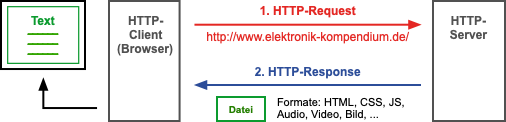
\includegraphics[width = 0.8\textwidth]{Sonne/HTTP-Client_Server_Kommunikation.jpg}
                    \caption{HTTP-Client-Server Kommunikation 
                    \cite{HTTP-Client_Server_Kommunikation}}
                    \label{HTTP-Client_Server_Kommunikation}
                \end{figure}
            
                \item \textbf{{OPC-UA (Open Platform Communications - Unified Architecture):}} \mbox{} \\
                Auch bei OPC UA gibt es Server und Clients. Dabei stellt der Server Daten bereit und die Clients können diese Daten abfragen oder Werte überschreiben. Dies ermöglicht einen sichere sowie zuverlässige Datenübertragung. 
                \cite{OPC-UA}
            \end{itemize}

            
    \paragraph{Welches Prorokoll wurde gewählt?} \mbox{} \\
    Bei diesem Projekt wurde das HTTP Protokoll ausgewählt um die Kommunikation zwischen SPS und Server auszuführen. Das HTTP Protokoll wurde ausgewählt, da die SPS direkt mit dem Server kommunizieren kann. Bei OPC-UA hätte ein zusätzlicher Server gehostet werden müssen. Dieser OPC-UA Server hätte dann mit dem eigentlichen Server, welcher die Lagerlogik übernimmt, kommuniziert. Die SPS hätte dann auf den OPC-UA Server zugegriffen und nicht direkt auf den Zielserver. Um diesen zusätzlichen Aufwand sowie weitere Fehlerquellen zu vermeiden, wurde das HTTP Protokoll ausgewählt.
        
            

    
    \subsubsection{Verbindungsherstellung}
    Aus den in Punkt \ref{Kommunikationsprotokolle} genannten Gründen wurde das HTTP Protokoll ausgewählt. Um in TIA-Portal die Verbindung via HTTP aufzubauen, benötigt man bestimmte Libraries die von Siemens zu Verfügung gestellt werden. Diese müssen dann wie im Punkt \ref{Bilbliotheken} gezeigt eingebunden werden, um die Funktionsbausteine der Library nutzen zu können. 

        \paragraph{Funktionsbausteine} \mbox{} \\
        In der Library für das HTTP Protokoll stehen dann folgende Bausteine zur Verfügung:

        \begin{itemize}
            \item GET
            \item POST-PUT 
        \end{itemize}
    
    Als Baustein zur Verbindungsherstellung wurde der POST-Befehl ausgewählt, da mit diesem unbegränzte Datenmengen geschickt werden können. Damit der Baustein nun eine Verbindung herstellen kann müssen folgende Parameter angegeben werden: \textbf{URL} [string], die zu schickenden Daten \textbf{data} [string] und ein Speicherplatz für die empfangenen Daten \textbf{response Data} [Array of Char]. Die restlichen Eingabeparameter, welche in Abb. \ref{POST-PUT_Baustein} ersichtlich sind,  müssen nicht unbedingt ausgefüllt werden, sondern werden automatisch vorausgefüllt. Standardmäßig ist die richtige Methode (POST) schon ausgewählt, da die Eingabe \textbf{method} automatisch mit \textbf{0} ausgefüllt wird. 

    \begin{figure} [h]
        \centering
        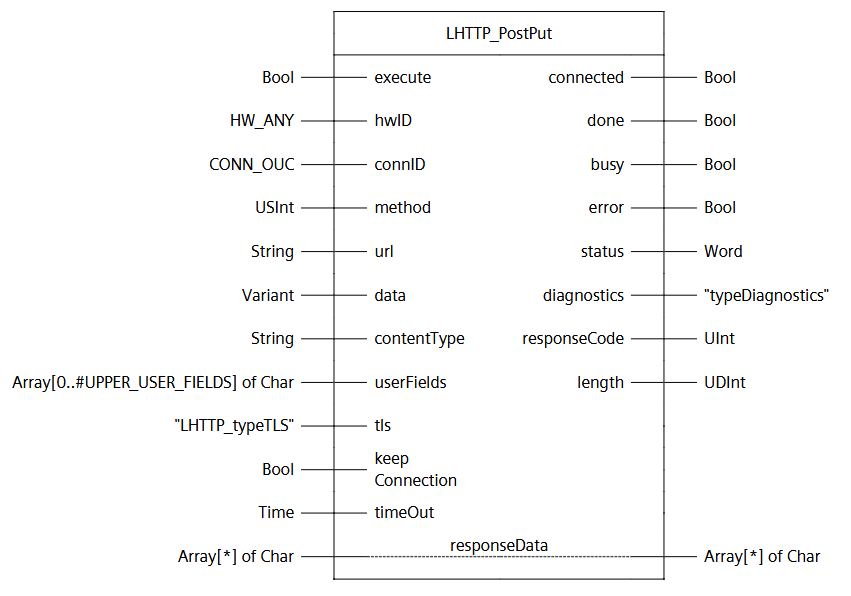
\includegraphics[width = 0.7\textwidth] {Sonne/POST-PUT_Baustein.png}
        \caption{POST-Put  Baustein \cite{HTTP-Bausteine}}
        \label{POST-PUT_Baustein}
    \end{figure}

    Wird nun die Eingabe \textbf{execute} HIGH, so wird der Baustein einmalig ausgeführt. Rechnet man mit einem häufigeren Datenaustausch, mit Hilfe dieses Bausteins, so empfiehlt es sich den Parameter \textbf{keep Connenction} auf \textbf{true} zu setzten. Dadurch bleibt die Verbindung mit dem Zielserver erhalten und weitere Kommunikationen werden dadurch schneller ausgeführt. 

    \subsubsection{Datenaustausch}
    Die SPS und der Server arbeiten mit verschiedenen Datentypen. Bei dem Datenaustauch erwartet der Server die Daten in einem json-Format. Deswegen müssen die Daten welche gesendet werden zuerst in dieses Format gebracht werden. Um dies in Tia-Portal zu realisieren wird die Bibilothek LStream eingebunden. Mit dieser werden dann Daten aus einem json-Datenbaum in ein Array of Byte umgewandelt. Dieses Array of Byte wird anschließend in den Datentyp string umgewandelt. Nun kann dieser string an den POST-Datenbaustein weitergegeben werden. \\
    Ist nun der Datenaustauch abgeschlossen, so sind die Daten als Array of Char verfügbar. Da man in Tia-Portal nur umständlich mit diesem Datenformat umgehen kann, wird das Array of Char nun in das Datenformat string umgewandelt. Die Daten sind nun noch immer nicht einzeln verfügbar, weswegen man nun diesen string nach den Daten filtern muss.

    \subsubsection{Datenfilterung}
    Die vom Server geschickten Daten werden in einem Befehl geschickt. Aus diesem Befehl muss herausgelesen werden um welche Aufgabe es sich handelt  und die Daten welche erforderlich sind um diese Aufgabe auszuführen.

        \paragraph{Datenformatierung}\mbox{}\\
        Die Daten werden in einem String geschickt, welcher in zwei Teile aufgeteilt wird. Der zweite Teil ist jedoch abhängig vom ersten. \\
        In folgenden Punkten dient x immer als Platzhalter für eine Nummer null bis neun. 
        \begin{itemize}
            \item 1.Teil: \\
            IDxxxxAxx  \\
            Aus diesem Teil werden die ID-Nummer sowie der Auftrag herausgefiltert. Die ID-Nummer ist eine 4 stellige Nummer welche nach ID steht. Der Auftrag welcher ausgeführt werden muss steht in den zwei Stellen nach A.\\
            Diese werden nach folgender Codierung ausgelesen:
                \subitem 00: Kommissionierstation
                \subitem 01: Förderband
                \subitem 10: Lager 1 (Aus-/Einlagerung)
                \subitem 11: Lager 1 (Querförderer)
            \item 2.Teil: \\
            Der zweite Teil steht in Abhängigkeit zu ersten. Je nachdem welche Zahl nach A steht,also der Code welche Area angesprochen wird, ist der zweite Teil anders aufgebaut.
                \begin{itemize}
                \item 00: SB\\
                Bei diesem Befehl muss der Barcodescanner angesteuert werden um an der Kommissionierstation einen Barcode einzuscannen.
                \item 01: P+-xxxx \\
                Gibt an um wie viel sich das Förderband bewegen muss [in mm]. Vor der Zahl steht jedoch entweder ein plus oder minus um festzulegen in welche Richtung sich das Förderband bewegen muss. 
                \item 10: XxxxxYxxxxZxxxxRx \\
                Nach jeder Achse X,Y,Z steht ein vierstelliger Wert, welcher angibt auf welcher Position sich der gewünschte Lagerplatz befindet. Der Wert nach R ist entweder 0 oder 1 und gibt an ob es sich um eine Einlagerung (1) oder Auslagerung (0) handet.
                \item 11: Pxxxx \\
                Nach P steht ebenso ein vierstelliger Wert, der angibt auf welche Position der Querförderer gefahren werden muss. 
                
                \end{itemize}
            
        \end{itemize}

\subsection{Herausforderungen}
